\chapter{Introduction}

Ultra-Low Power Processors, such as ARM's Cortex-M0+, are becoming an increasingly appealing area of research, particularly because they provide a platform for the Internet of Things. As our culture develops new ways for technology to aid our every-day lives, the devices which support these progressions are required to be less and less intrusive, forcing companies to search for new methods of making systems smaller and require lower power, especially as ``essentially all IoT sensor nodes will be powered by small batteries and to a lesser extent by energy harvesting'' \cite{iot_power}.

However, such processors clearly create very tight constraints for potential developers, as processing power is often limited, leading to the ever-continuing requirement for more efficient and optimised algorithms. As memory usage is also proportional to power consumption, the RAM available on such systems is extremely limiting. As we begin to rely on these systems more and more, these constraints make it a growing challenge to implement systems which are not only useful, but can be relied upon to function when needed. This is particularly important in cases in which a device is being used for safety-critical operations, which is becoming increasingly common \cite{iot_saftey} \cite{iot_saftey2}.

ARM is currently investigating the concept of a sub threshold Cortex-M0+ \cite{arm_sub}, which attempts to push the extremes of these constraints further by providing just 8 kB of memory for both program code and data, and running at just a few hundred kHz. This project aims to research and develop an algorithm which is capable of running on such a device, to act as a proof of concept that such a processor would be worthwhile.

\namedsection{Project Overview}{Finch}

The particular algorithm that the group developed is a way to identify and monitor exercises performed by a human wearer. These are specifically exercises which can be done on aeroplanes to reduce the risk of suffering from Deep Vein Thrombosis, a condition where a blood clot can form in one of the deep veins in the body, most commonly the legs. This can lead to further complications such as pulmonary embolism which occurs when part of the blood clot moves and blocks a blood vessel in the lungs \cite{dvt}. Long-haul flights can increase the risk of getting DVT because of the long periods of time sitting down and not moving which reduces circulation in the legs.

\begin{figure}[h]
  \centering
    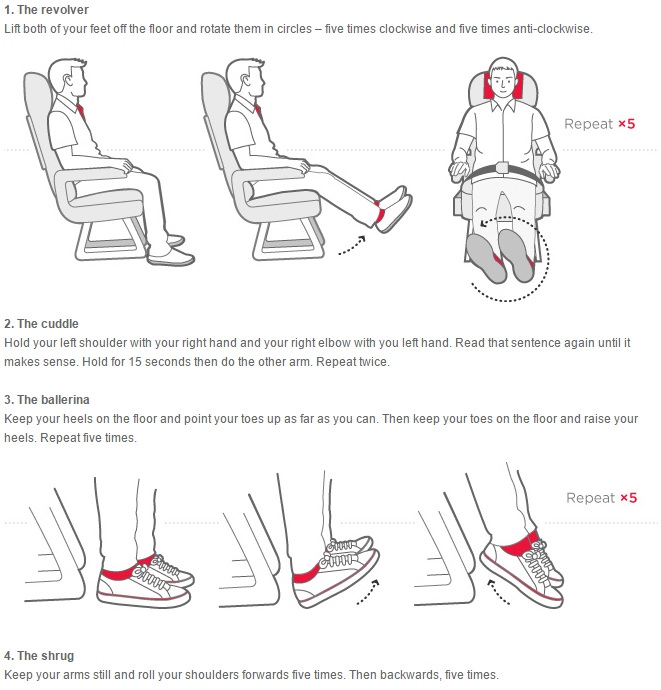
\includegraphics[width=1.0\textwidth]{figures/exercises}
  \caption{In-flight exercises \cite{virgin2015exercises}}
  \label{fig:exercises}
\end{figure}

Figure \ref{fig:exercises} shows some of the in-flight exercises which can be performed. We have looked into a few of them including the revolver, the ballerina and the shrug. These involve lifting both feet off the floor and rotating them in circles in clockwise and anticlockwise directions, pointing the feet up and down and rolling the shoulders backwards and forwards. These are all designed to help keep the circulation going in the limbs. However, a specific focus was made to the revolver exercise for the purpose of prototyping a system.

Possible uses of the algorithm would be to incorporate it into a device which could be given to passengers to strap to their legs. It would then monitor how much exercise each person was doing. This could help inform the passengers whether or not they are doing enough exercise to stay risk free. The device itself could make use of energy efficient technologies (for example the Cortex-M0+) so that its battery could easily last the entire duration of a long-haul fight.

\namedsection{Project Requirements }{Finch}

The main requirement of this project is to develop an algorithm which is capable of detecting and monitoring exercises on a sub threshold Cortex-M0+. This processor is clocked at 100 kHz, although it can increase to 3 MHz if required. However, the lower the clock speed the better as this would clearly require less power.

Additionally, 8 kB is imposed as the memory limit for both program code and data in order for the algorithm to be capable of running on the sub threshold Cortex-M0+. Again, the lower this can be the better as it opens up the possibility for the system to require even less power.

As the proposed sub threshold Cortex-M0+ is still in development, it is not readily available for the group to use; consequently, the team was required to investigate alternatives to emulate the processor. These alternatives must allow the clock speeds to be adjusted based on the efficiency and requirements of the algorithm. The challenges involved in this are discussed in chapter~\ref{chap:embedded}.

Research and analysis of the algorithms used for exercise detection which currently exist, specifically focusing on Machine Learning techniques, was also carried out. On top of this, an investigation into the tools and techniques which can be used, along with the methods by which the effectiveness of trained algorithms can be evaluated was also necessary. This is documented in chapter~\ref{chap:research}.

Following on from this, the ways in which the algorithm can be optimised to run on a such constrained system must also be explored. The way this was done is examined in chapter~\ref{chap:software}.

Another requirement of the project was to perform a user study to collect movement data of the exercises which can be used to develop the algorithm. This is so that a range of data from a selection of different people can be used because each individual is likely to perform the exercises with slight variations. The details of this can be found in chapter~\ref{chap:study}.

Finally, the accuracy of the developed algorithm is calculated; the specifics of this are outlined in chapter~\ref{chap:results}.
Below, the requirements of this project are given in explicit detail.

\namedsection{Detailed Requirements}{Finch}

\begin{enumerate}
  \item The algorithm must be capable of detecting and monitoring exercises designed to combat deep vein thrombosis
  \begin{enumerate}[label*=\arabic*.]
    \item These are exercises which can be performed in a plane, particularly in long haul flights and include:
    \begin{enumerate}[label*=\arabic*.]
      \item Foot rotations
      \item Pointing feet up and down
      \item Shoulder rolling
    \end{enumerate}
    \item Other activities such as walking should be distinguished as not being exercise
  \end{enumerate}
  \item The algorithm must be suitable to execute on an ultra-low-power sub threshold ARM Cortex-M0+
  \begin{enumerate}[label*=\arabic*.]
    \item This device has a limited processor clocked from 100 kHz to a maximum of 3 MHz
    \item Memory usage should be kept to a minimum with a target of no more than 8 kB
    \item Therefore, the algorithm should be highly optimised to use as little memory and require as little processing power as possible
  \end{enumerate}
  \item The sub threshold Cortex-M0+ must be emulated in a test platform as working with the actual M0+ is not feasible
  \begin{enumerate}[label*=\arabic*.]
    \item The test platform should be capable of being clocked at frequencies ranging from only a 100 kHz to 3 MHz
    \item The test platform should have at least 32 kB of memory to aid with testing and to act as a fall back if 8 kB cannot be achieved
    \item There must be an accelerometer sensor on the platform that readings can be taken from
  \end{enumerate}
  \item Research into various potential algorithms must take place
  \begin{enumerate}[label*=\arabic*.]
    \item Machine learning approaches should be focussed on
    \item Algorithms which are used on unconstrained systems should be considered first
    \item The feasibility of constraining those algorithms should then be investigated
    \item The methods of evaluating algorithm performance should also be examined
  \end{enumerate}
  \item Participant studies should be performed to gather movement data to train the algorithm
  \begin{enumerate}[label*=\arabic*.]
    \item Ethics approval will need to be obtained
  \end{enumerate}
  \item The developed algorithm must be deployed to the test platform
  \item The final system must then be evaluated in terms of its accuracy at detecting exercises
\end{enumerate}
